\section{Results}
\label{sec:results}

Looking at Figure \ref{fig:hovmollerSinePeriodic}, we observe the time evolution of a sine wave in the periodic domain. We see that the wave is easterly (travelling towards the west). There are four distinct anti-nodes throughout the entire duration of the wave, and a wavelength is determined to be $0.5$. After a time $t=80$ we can see that the wave is in phase to its initial state.
\begin{figure}[htbp]
	\centering
	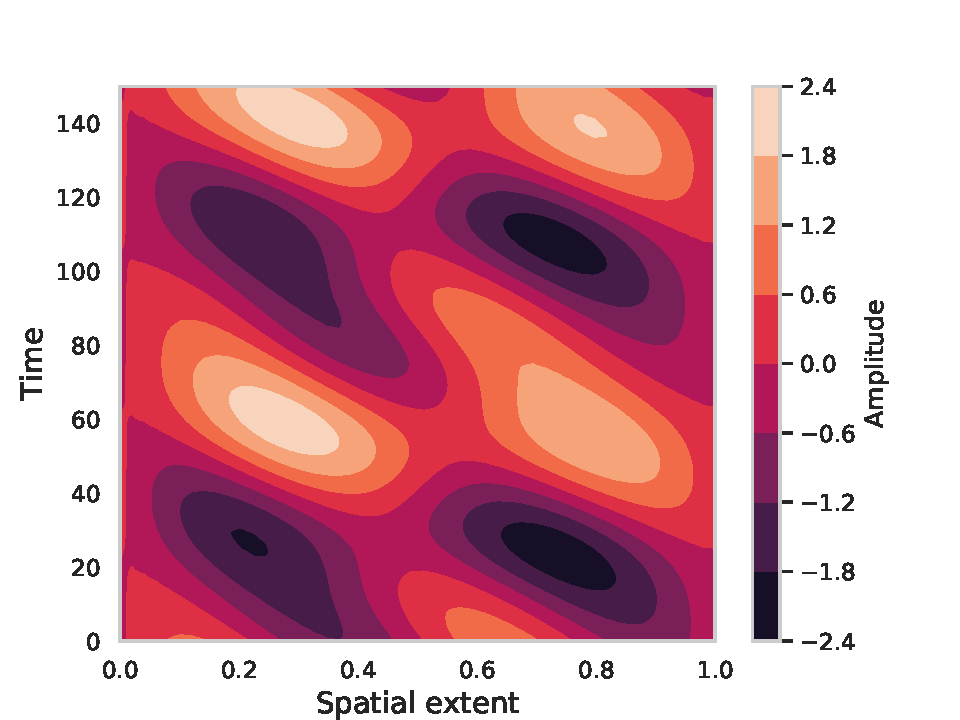
\includegraphics[width=0.5\textwidth]{hovmuller_periodicsine.pdf}
	\caption{Hovmöller diagram of a Rossby wave with \textbf{periodic} boundary conditions, initially a sine wave using a implicit scheme, where $\Delta x = 0.025$ and $\Delta t = 0.1$.}
	\label{fig:hovmollerSinePeriodic}
\end{figure}

Considering now the bounded sine wave (Figure \ref{fig:hovmollerSineBounded}), the direction of propagation is still west. The shape of the curve appears to be the same as for the periodic case, except that the equilibrium line of the sine curve is shifting up and down, so that the boundary conditions are satisfied.
\begin{figure}[htbp]
	\centering
	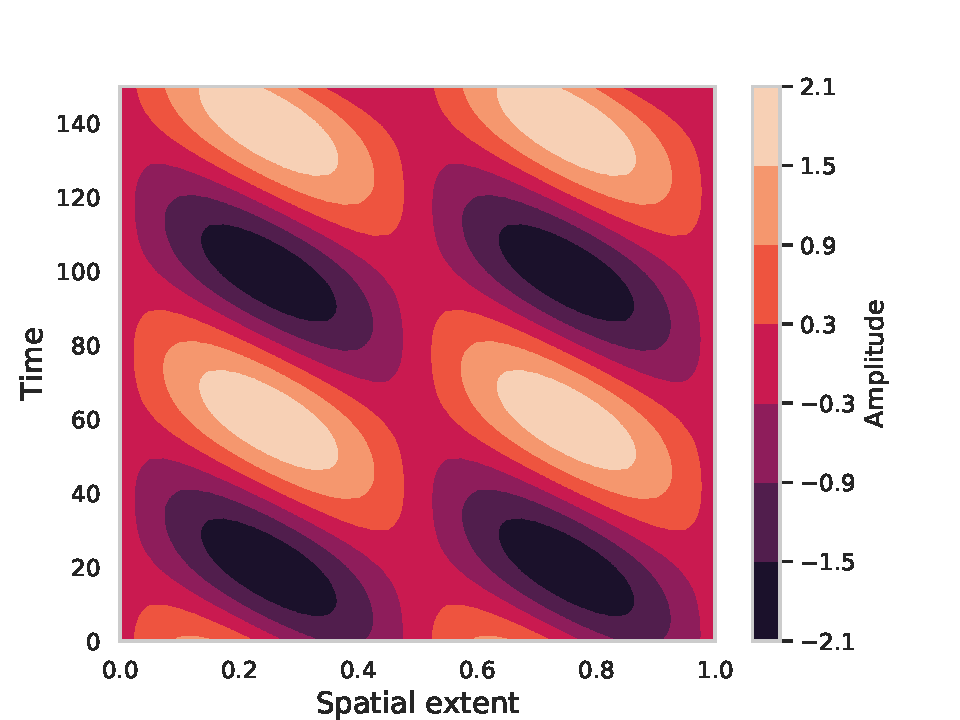
\includegraphics[width=0.5\textwidth]{hovmuller_boundedsine.pdf}
	\caption{Hovmöller diagram of a \textbf{bounded} Rossby wave with a initial sine wave using a implicit scheme. Here $\Delta x = 0.025$ and $\Delta t = 0.1$.}
	\label{fig:hovmollerSineBounded}
\end{figure}

From Figure \ref{fig:hovmollerGaussianPeriodic005}, \ref{fig:hovmollerGaussianPeriodic} and \ref{fig:hovmollerGaussianPeriodic015}, we see that, in general, the periodic gaussian wave exhibits different behaviour compared to the sine wave. There are at most two distinct anti-nodes at any point in time, and there looks to be a changing pattern in time, compared to the sine waves which always look the same. For varying width, $\sigma$, we see that the location of the anti-node are more concentrated in the middle for lower $\sigma$ (Figure \ref{fig:hovmollerGaussianPeriodic005}) and more spread out for higher $\sigma$ (Figure \ref{fig:hovmollerGaussianPeriodic015}).
\begin{figure}[htbp]
	\centering
	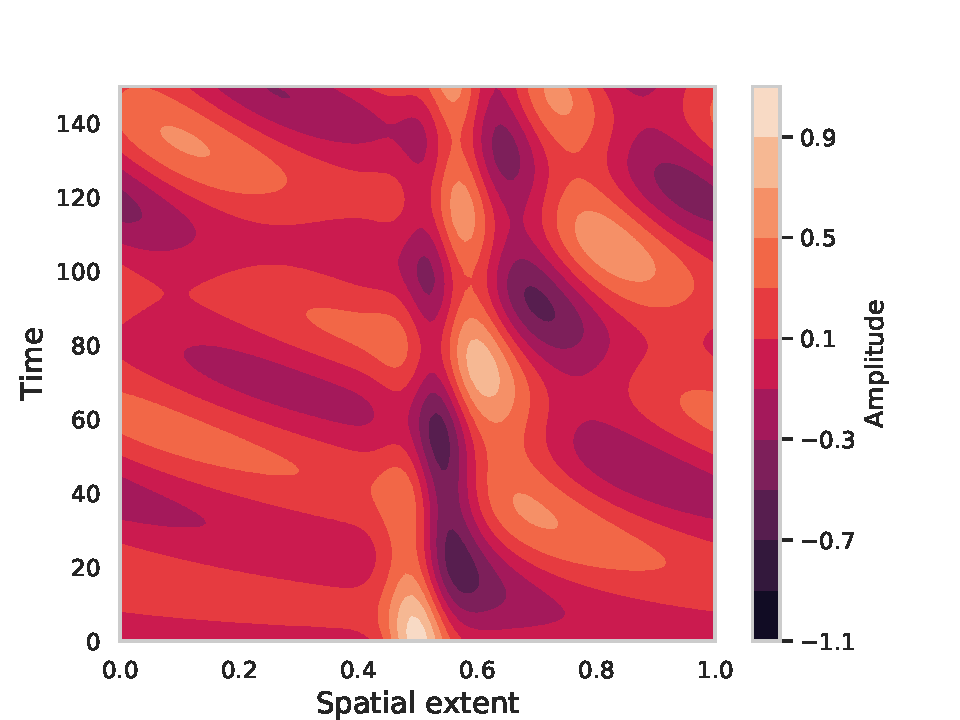
\includegraphics[width=0.5\textwidth]{hovmuller_periodicgaussian_sigma005.pdf}
	\caption{Hovmöller diagram of a Rossby wave with \textbf{periodic} boundary conditions, initially a centered gaussian ($x_0=0.5$) using a implicit scheme. Here $\sigma = 0.05$, $\Delta x = 0.01$ and $\Delta t = 0.1$.}
	\label{fig:hovmollerGaussianPeriodic005}
\end{figure}

\begin{figure}[htbp]
	\centering
	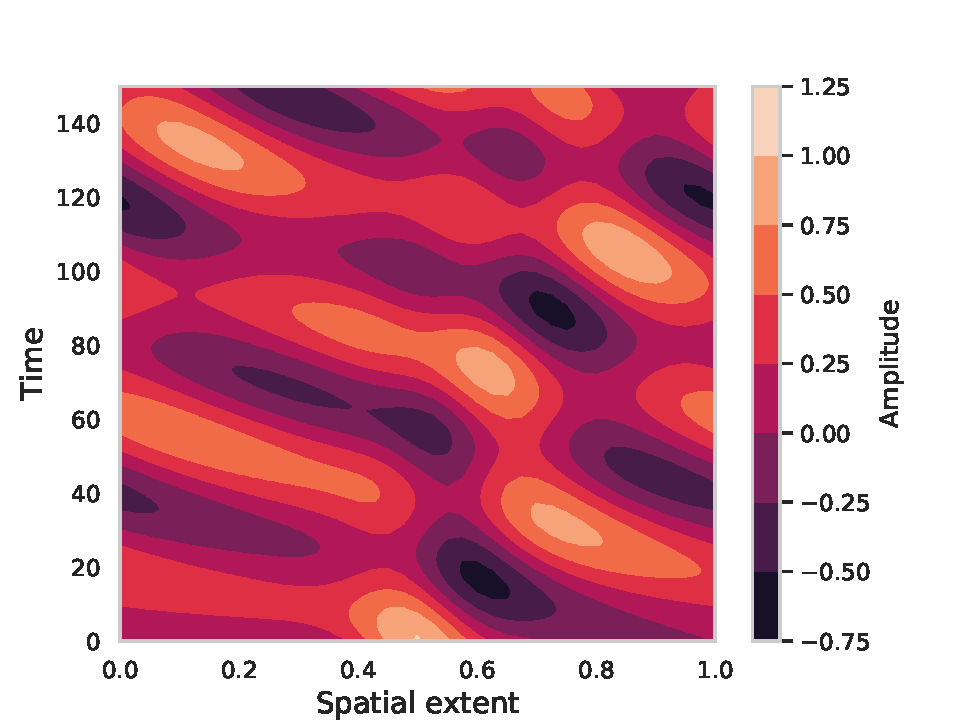
\includegraphics[width=0.5\textwidth]{hovmuller_periodicgaussian.pdf}
	\caption{Hovmöller diagram of a Rossby wave with \textbf{periodic} boundary conditions, initially a centered gaussian ($x_0=0.5$) using a implicit scheme. Here $\sigma = 0.1$, $\Delta x = 0.025$ and $\Delta t = 0.1$.}
	\label{fig:hovmollerGaussianPeriodic}
\end{figure}

\begin{figure}[htbp]
	\centering
	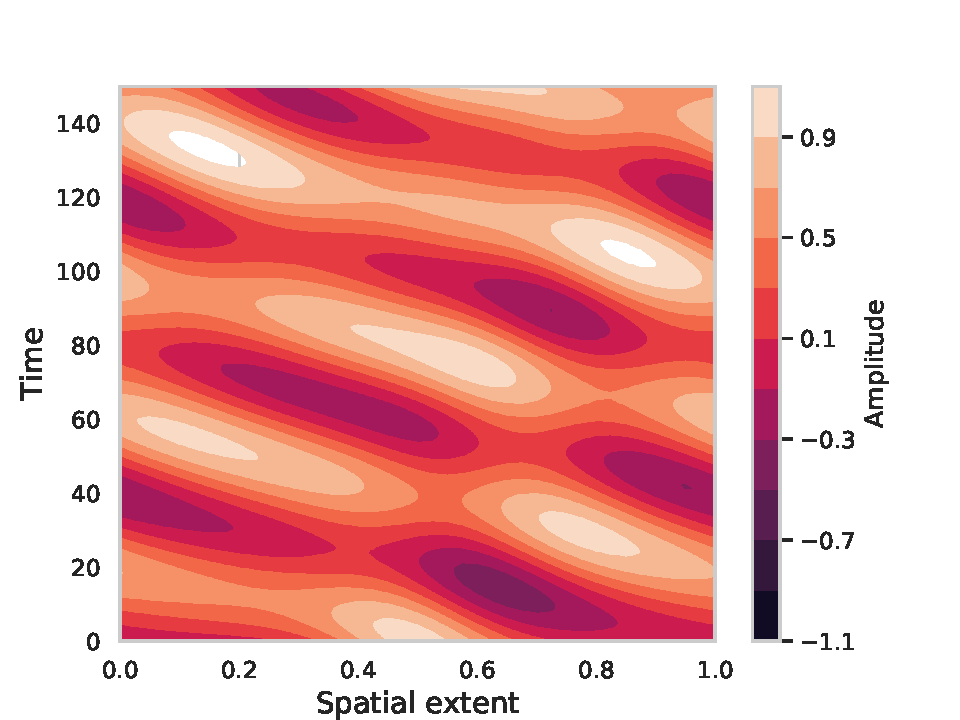
\includegraphics[width=0.5\textwidth]{hovmuller_periodicgaussian_sigma015.pdf}
	\caption{Hovmöller diagram of a Rossby wave with \textbf{periodic} boundary conditions, initially a centered gaussian ($x_0=0.5$) using a implicit scheme. Here $\sigma = 0.15$, $\Delta x = 0.025$ and $\Delta t = 0.1$.}
	\label{fig:hovmollerGaussianPeriodic015}
\end{figure}

In Figure \ref{fig:hovmollerGaussianBounded} we show the Hovmöller diagram of a gaussian with closed boundaries. In this case, while there are still variations in time, we can clearly discern oscillations between minima and maxima.
\begin{figure}[htbp]
	\centering
	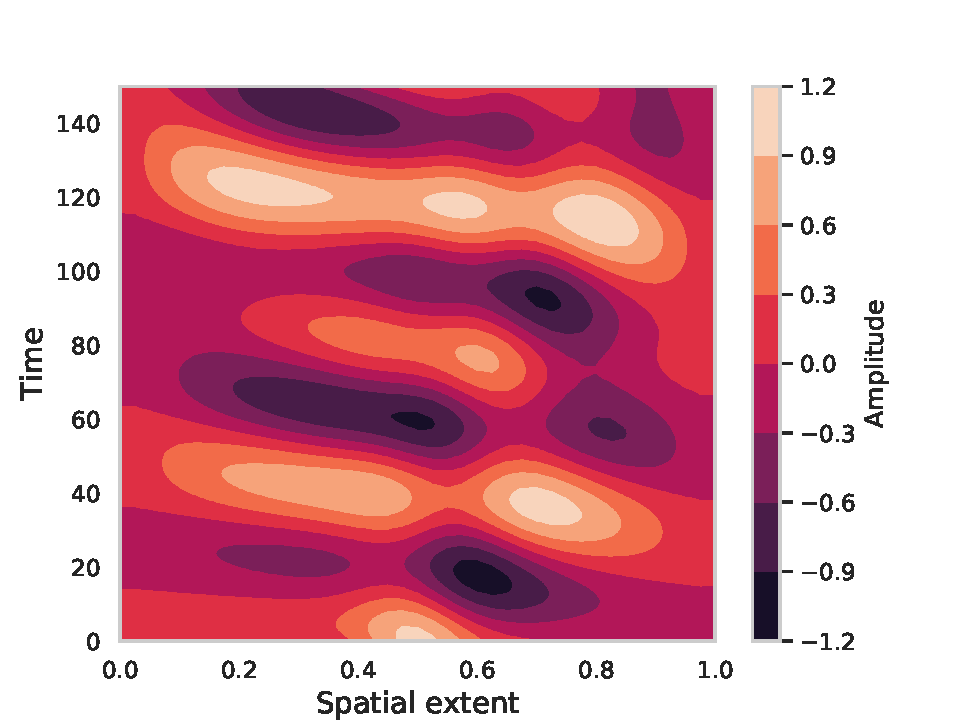
\includegraphics[width=0.5\textwidth]{hovmuller_boundedgaussian.pdf}
	\caption{Hovmöller diagram of a \textbf{bounded} Rossby wave initially a centered gaussian ($x_0=0.5$) using a implicit scheme. Here $\sigma = 0.1$, $\Delta x = 0.025$ and $\Delta t = 0.1$.}
	\label{fig:hovmollerGaussianBounded}
\end{figure}

Figure \ref{fig:boundedsine2d} and \ref{fig:periodicsine2d} shows the evolution of an initial product between two sine waves, one in the x-direction and one in the y-direction, resulting in an two dimensional wave, for four different time steps, both in a periodic and bounded domain. In the periodic domain, the wave seems to keep its structure, while shifting in the x-direction. The direction can not be derived solely from these four time steps. However, referring to the code for animating the time evolution found in the GitHub repository janadr/FYS3150/prosjekt5/kode, it can be seen that the wave is travelling to the left. It should be noted that due to a lack of time, the code used to generate the data shown in Figure \ref{fig:periodicsine2d} does not handle the eastward boundary correctly. 

For the bounded two dimensional domain, the amplitude of the wave have decreased closer to the x-boundaries for the time steps $t\neq 0$. Again it can be seen from the mentioned animation program that the wave is travelling westward. 
\begin{figure}[htbp]
	\centering
	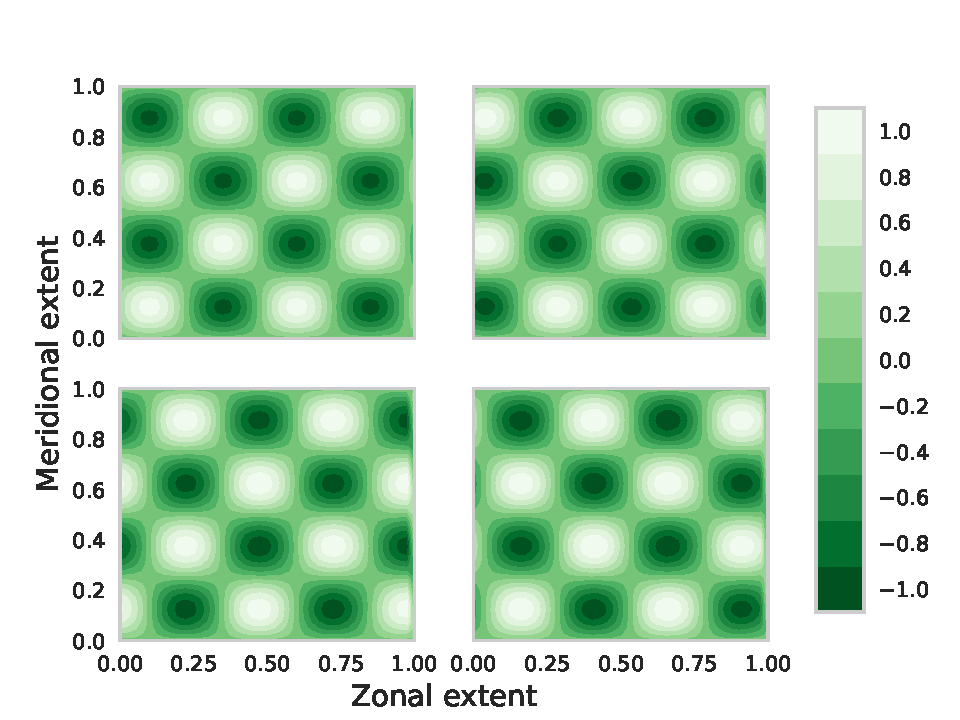
\includegraphics[width=0.5\textwidth]{periodic_sine_centered_2d.pdf}
	\caption{2+1 dimensional time evolution of a sine wave in the \textbf{periodic} domain, where time advances from left to right, top to bottom, for $t = 0,\, 50,\, 100,\, 150$ respectively. Here $\Delta x = 0.025$ and. $\Delta t = 0.1$}
	\label{fig:periodicsine2d}
\end{figure}

\begin{figure}[htbp]
	\centering
	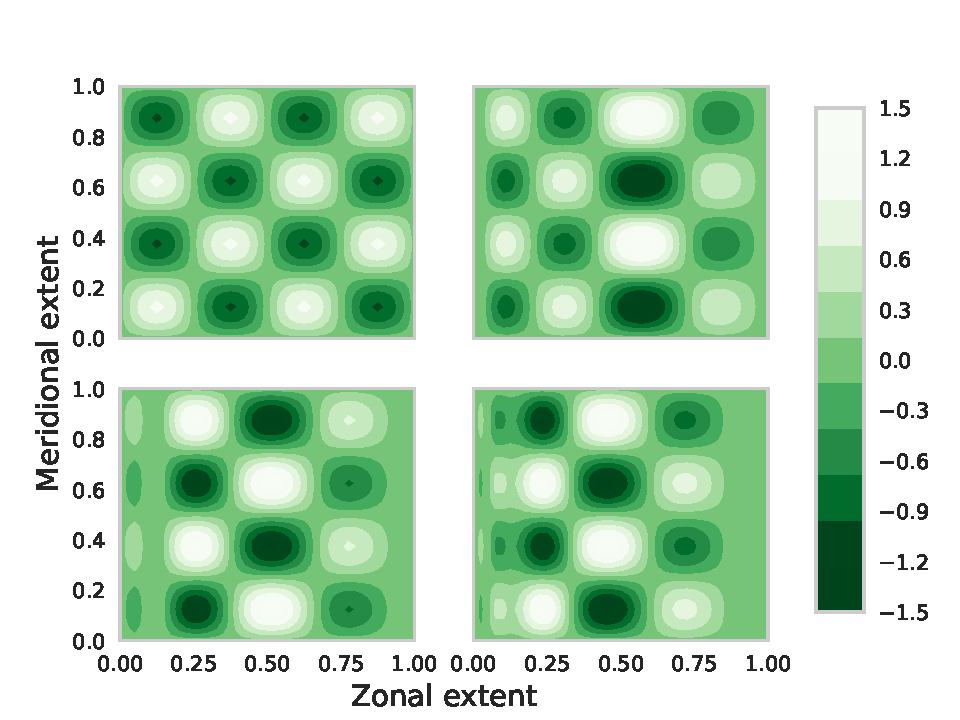
\includegraphics[width=0.5\textwidth]{bounded_sine_centered_2d.pdf}
	\caption{2+1 dimensional time evolution of a sine wave in the \textbf{bounded} domain, where time advances from left to right, top to bottom, for $t = 0,\, 50,\, 100,\, 150$ respectively. Here $\Delta x = 0.025$ and. $\Delta t = 0.1$}
	\label{fig:boundedsine2d}
\end{figure}


